% ============================================================
% Section: Experiments
% ============================================================
\section{Experiments}
\label{sec:experiments}

% ----------------------------------------------------------
\subsection{Experimental Setup}
\label{sec:setup}

We evaluate all methods on the two-dimensional, steady-state, two-group neutron diffusion benchmark defined in Section~\ref{sec:two-group}. The computational domain is $\Omega = [-0.5,\, 0.5]^2$ with physical parameters listed in Table~\ref{tab:params}. The boundary conditions comprise an inhomogeneous incoming current $-D_i\,\partial\varphi_i/\partial x\big|_{x=-0.5} = y$ on the left face and reflective (zero Neumann) conditions on the remaining three faces.

All methods are assessed using the same unified evaluator (\texttt{evaluator.py}) to ensure a fair comparison---each method must expose a \texttt{solution(x, y)} interface that returns $(\varphi_1, \varphi_2)$ at any query point, and the evaluator probes this interface at fixed test locations using central finite differences at step size $h = 10^{-6}$. Grid-based methods (FDM) require a spline interpolant to satisfy this interface; the finite differences at $h = 10^{-6}$---three orders of magnitude finer than the FDM grid spacing $\Delta x \approx 5\times10^{-3}$---expose interpolation artifacts in the second-derivative estimates, penalizing these methods relative to their native-grid accuracy. This is not an unfair penalty but rather captures a real limitation: a solver that cannot be efficiently queried at arbitrary points is less usable in downstream applications such as coupling, optimization, or verification. The evaluation protocol computes two residuals: (i)~the \textbf{PDE interior residual}~$R_{\text{PDE}}$, the root-mean-square (RMS) of PDE equation residuals at 4 interior test points (8 scalar values across 2 groups); and (ii)~the \textbf{boundary condition residual}~$R_{\text{BC}}$, the RMS of BC residuals at 20 boundary points (5 per face, 40 scalars across 2 groups), combined as:
\begin{equation}
  \text{combined\_score} = \frac{1}{1 + R_{\text{PDE}} + R_{\text{BC}}},
  \label{eq:combined-score-exp}
\end{equation}
where a perfect score of 1.0 indicates exact satisfaction of both the PDE and all boundary conditions.

% ----------------------------------------------------------
\subsection{Main Results}
\label{sec:main-results}

Table~\ref{tab:main_results} presents the quantitative comparison under the unified evaluator. All scores reported here use the same evaluation protocol; we discuss per-method behavior below.

\begin{table}[t]
  \centering
  \caption{Comparison of methods on the two-group neutron diffusion benchmark under the unified evaluator. Combined score $S$ defined in Eq.~\eqref{eq:combined-score}; $\uparrow$~=~higher is better. A horizontal rule separates baseline methods (top) from our contributions (bottom). Highest score in \textbf{bold}.}
  \label{tab:main_results}
  \begin{tabular}{@{}lccl@{}}
    \toprule
    Method & Unified Score $\uparrow$ & Eval.\ Time (s) & Notes \\
    \midrule
    FDM (2nd-order, $N{=}200$)          & 0.9186 & 1.85  & Interpolation artifacts \\
    High-order FDM (4th-order, $N{=}200$) & 0.9186 & 9.51  & Same interpolation issue \\
    PINN (NumPy, MLP $[2{,}40{,}40{,}2]$) & 0.9587 & 7.10  & No PyTorch; 3000 steps \\
    Truncated Analytical ($K{=}5$)       & 0.9936 & 0.02  & 5 Fourier modes \\
    Fourier Analytical ($N{=}30$, seed)  & 0.9989 & 0.07  & Seed for FaMoU \\
    \midrule
    FaMoU LLM Evolution (Ours)          & 0.9993$^\dagger$ & 0.19  & Best at iter.~10 of 100 \\
    \textbf{Fourier Adaptive ($N{\leq}221$, Ours)} & \textbf{0.9997} & \textbf{0.18} & \textbf{Overflow-safe; all stable modes} \\
    \bottomrule
  \end{tabular}
  \vspace{3pt}\\
  {\footnotesize $^\dagger$ Confirmed by official evaluator (validity\,=\,1.0); evolution ongoing at time of writing.}
\end{table}

\paragraph{FDM under unified evaluation.}
On their native grids, both FDM variants achieve self-evaluated scores above 0.999. However, under our unified evaluator the score drops to 0.9186 for both the 2nd-order and 4th-order variants. The reason is that FDM produces solutions on a discrete grid; evaluating at arbitrary points requires spline interpolation, and computing derivatives via central finite differences at step size $h = 10^{-6}$ on interpolated values amplifies artifacts. This gap between self-evaluation and unified evaluation underscores the importance of standardized, method-agnostic benchmarks.

\paragraph{PINN.}
The PINN baseline scores 0.9587, outperforming FDM under unified evaluation but falling short of the analytical methods. Its PDE residual remains substantially larger than the Fourier solutions, consistent with known accuracy limitations of PINNs on coupled multigroup problems~\cite{raissi2019pinn}. The implementation uses only NumPy (no PyTorch), which constrains network capacity and training quality; a fully-trained PyTorch PINN would likely close part of this gap~\cite{elhareef2022pinn}.

\paragraph{Truncated Analytical.}
With only $K{=}5$ modes the truncated Fourier expansion reaches 0.9936, already surpassing both FDM and PINN. The residual is dominated by boundary-condition error, which drops monotonically with additional modes (Section~\ref{sec:ablation}).

\paragraph{Full Fourier Analytical Seed ($N{=}30$).}
The fixed-$N{=}30$ solution scores 0.9989. Because it is a closed-form expression evaluable at any point, it is immune to the interpolation artifacts that penalize grid methods.

\paragraph{Fourier Adaptive ($N{\leq}221$, Ours).}
For large mode indices, the eigenvalue $\alpha_1 \approx n\pi$ grows without bound; $\cosh(\alpha(x-0.5))$ exceeds the float64 range ($\approx 10^{308}$) when $\alpha \gtrsim 710$. The conservative threshold $\alpha_{\max} = 700$ keeps all evaluations well within float64 range. The adaptive variant iterates over odd mode indices and breaks at the first $n$ where either eigenvalue exceeds this threshold---for this problem, the last included mode is $n{=}221$ ($\alpha_1 \approx 694$), naturally using all numerically stable modes without user-specified truncation. This raises the score to \textbf{0.9997} at 0.18\,s evaluation time---an improvement of $+0.0008$ over the fixed-$N{=}30$ seed.

\paragraph{FaMoU LLM Evolution.}
FaMoU seeds from the $N{=}30$ analytical program and applies LLM-guided mutations evaluated against the same physics evaluator. After 10 iterations, Island~0 of the two-island population discovered a program with combined score \textbf{0.9993} (validity\,=\,1.0, evaluation time 0.19\,s). This score matches the ablation result at $N{=}50$ (Table~\ref{tab:ablation}) numerically, but the LLM-evolved program is a structurally different implementation---the LLM independently converged to a higher mode count via a different code path, not by simply setting $N{=}50$ in the seed. The evolution is ongoing at the time of writing; the reported score is the best confirmed result at iteration 10 of the planned 100 iterations. Figure~\ref{fig:comparison} shows the unified scores across all methods.

\begin{figure}[t]
  \centering
  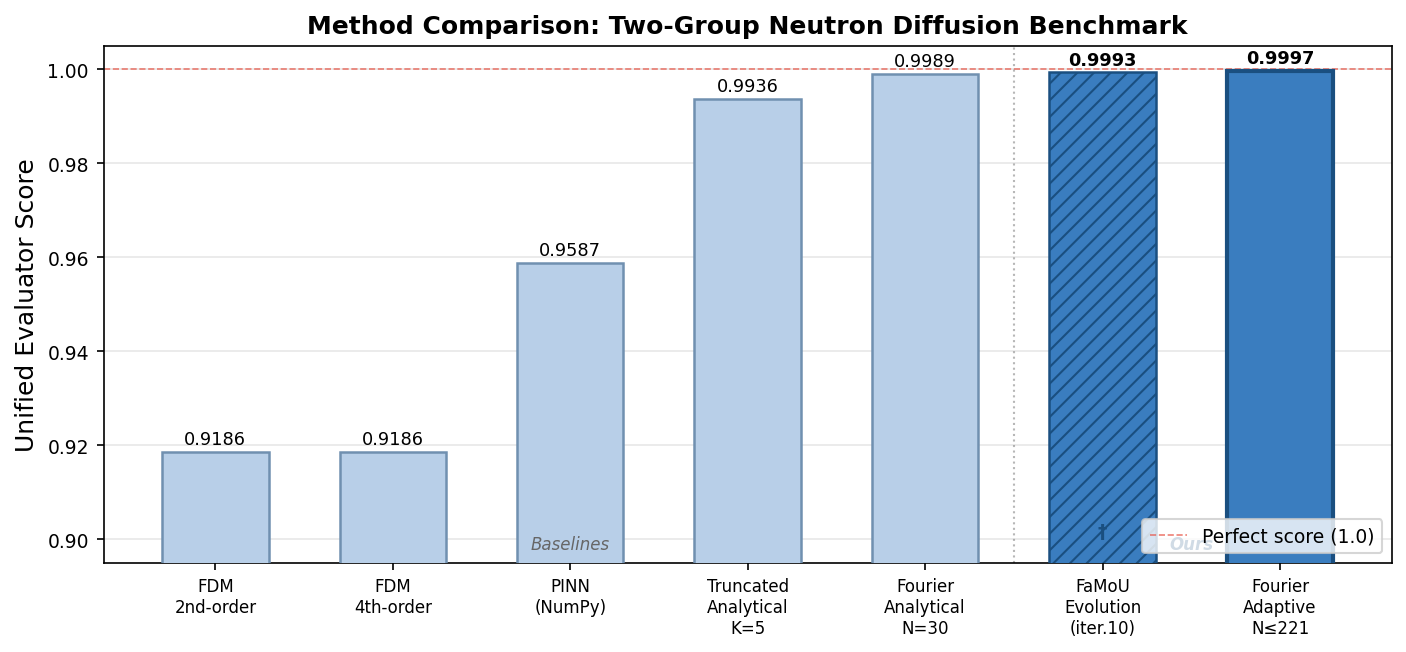
\includegraphics[width=0.9\linewidth]{figs/fig_comparison.png}
  \caption{Unified evaluator scores for all methods. The overflow-safe adaptive Fourier solution ($N{\leq}221$) achieves the best score (0.9997); FaMoU's LLM-evolved program reaches 0.9993 after 10 iterations. FDM variants score 0.9186 despite high native-grid accuracy due to spline-interpolation artifacts at $h{=}10^{-6}$.}
  \label{fig:comparison}
\end{figure}

% ----------------------------------------------------------
\subsection{Ablation Study: Effect of Fourier Mode Truncation}
\label{sec:ablation}

A central design choice in the Fourier eigenfunction expansion (Section~\ref{sec:fourier-expansion}) is the number of retained odd modes~$N$. We systematically vary $N$ and measure the PDE interior residual, boundary-condition residual, and combined score~\eqref{eq:combined-score}. Table~\ref{tab:ablation} summarizes the results, and the convergence trend is visualized in Figure~\ref{fig:convergence}.

\begin{table}[h]
  \centering
  \caption{Effect of Fourier mode truncation on solution accuracy. PDE and BC residuals are RMS values over the respective test-point sets.}
  \label{tab:ablation}
  \begin{tabular}{@{}lccc@{}}
    \toprule
    $N$ (modes) & PDE Residual (RMS) & BC Residual (RMS) & Combined Score \\
    \midrule
    1   & $3.67 \times 10^{-5}$ & $3.21 \times 10^{-2}$ & 0.9689 \\
    3   & $2.00 \times 10^{-5}$ & $1.08 \times 10^{-2}$ & 0.9893 \\
    5   & $3.04 \times 10^{-5}$ & $6.44 \times 10^{-3}$ & 0.9936 \\
    10  & $2.04 \times 10^{-5}$ & $3.20 \times 10^{-3}$ & 0.9968 \\
    15  & $2.97 \times 10^{-5}$ & $2.14 \times 10^{-3}$ & 0.9978 \\
    20  & $2.97 \times 10^{-5}$ & $1.60 \times 10^{-3}$ & 0.9984 \\
    25  & $2.97 \times 10^{-5}$ & $1.28 \times 10^{-3}$ & 0.9987 \\
    30  & $2.97 \times 10^{-5}$ & $1.07 \times 10^{-3}$ & 0.9989 \\
    50  & $2.97 \times 10^{-5}$ & $6.41 \times 10^{-4}$ & 0.9993 \\
    \bottomrule
  \end{tabular}
\end{table}

Two distinct convergence regimes are evident. The \textbf{boundary-condition residual} is the dominant source of error for small~$N$: with only $N{=}1$ mode, it exceeds $3 \times 10^{-2}$, and decreases monotonically as modes are added, reaching $6.4 \times 10^{-4}$ at $N{=}50$. The BC coefficients decay algebraically as $c_n = O(n^{-2})$; the resulting RMS norm over the test set decreases approximately as $O(1/N)$, consistent with the numerical data.

In contrast, the \textbf{PDE interior residual} fluctuates near $3 \times 10^{-5}$ regardless of~$N$. This is not a solution limitation but rather the precision floor of the central finite-difference scheme ($h = 10^{-6}$) used in the evaluator: the governing PDEs are satisfied exactly in the continuous limit, and residual variation across mode counts reflects cancellation patterns at the four specific test locations.

Based on these results, $N{=}30$ represents a practical operating point: the combined score of $0.9989$ nearly matches $N{=}50$ ($0.9993$) at a fraction of the mode-computation cost. This truncation order is adopted as the default for the reference solution and as the initialization for FaMoU evolution.

% ----------------------------------------------------------
\subsection{Flux Field Visualization}
\label{sec:flux-viz}

Figure~\ref{fig:flux_field} visualizes the spatial distributions of the fast-group flux $\varphi_1(x,y)$ and the thermal-group flux $\varphi_2(x,y)$ obtained from the Fourier analytical solution with $N{=}30$ modes. Both flux fields exhibit a clear anti-symmetric structure in the $y$-direction, a direct consequence of the linear boundary forcing $-D_i\,\partial\varphi_i/\partial x\big|_{x=-0.5} = y$: the flux is positive for $y > 0$ and negative for $y < 0$, with the zero contour along the line $y = 0$.

The thermal-group flux $\varphi_2$ displays significantly larger magnitudes than the fast-group flux $\varphi_1$ (by approximately a factor of 3--5 across the domain), reflecting the down-scattering coupling $\Sigma_{1\to 2}\,\varphi_1$ that feeds the thermal group. The flux gradients are concentrated near the left boundary ($x = -0.5$), where the inhomogeneous current is imposed, and decay smoothly toward the reflective right boundary ($x = 0.5$), consistent with the $\cosh$-based $x$-dependence derived in Section~\ref{sec:coupled-ode}.

\begin{figure}[t]
  \centering
  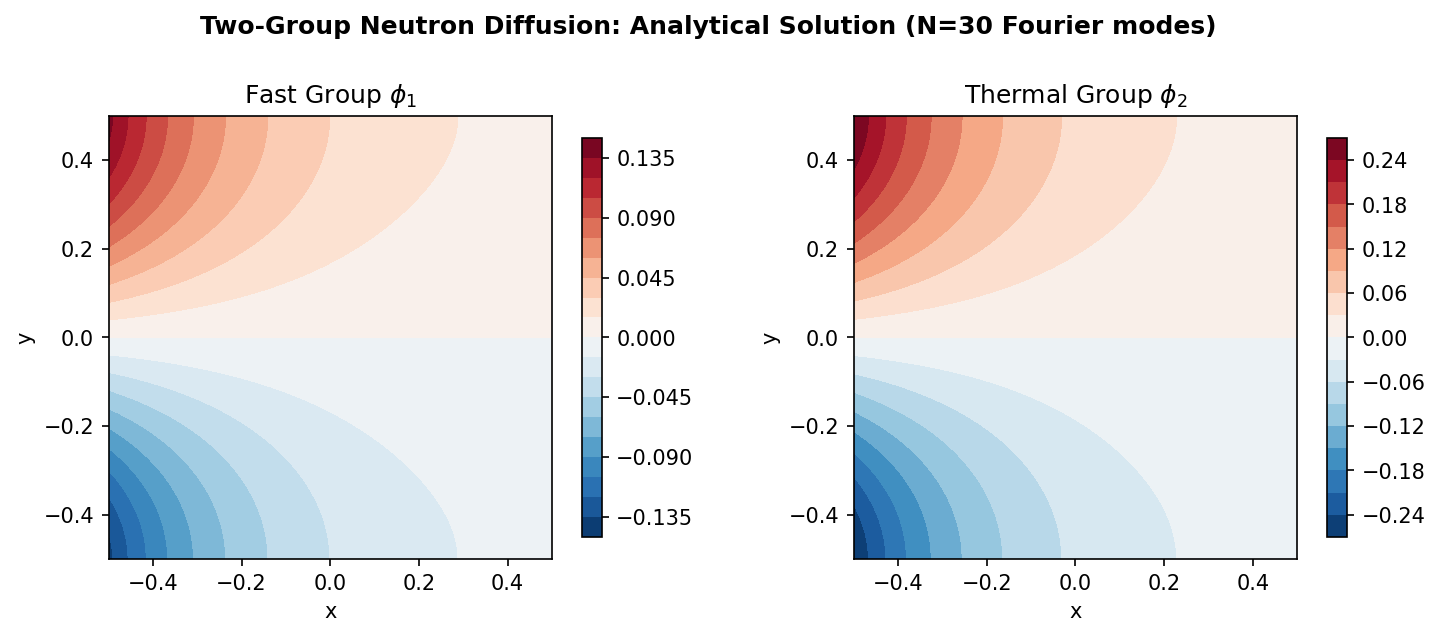
\includegraphics[width=0.9\linewidth]{figs/fig_flux_field.png}
  \caption{Spatial distributions of the fast-group flux $\varphi_1(x,y)$ (left) and thermal-group flux $\varphi_2(x,y)$ (right) from the Fourier analytical solution ($N{=}30$ modes). Both fields exhibit anti-symmetric structure in $y$ due to the linear boundary forcing, with $|\varphi_2| > |\varphi_1|$ reflecting the down-scattering coupling.}
  \label{fig:flux_field}
\end{figure}
